\begin{frame}
\frametitle{Smart scheduling approach for EVs}

\begin{PraesentationAufzaehlung}
    \item \textbf{paper:} ``Smart Charging Schedules for Highway Travel with Electric Vehicles''
        \begin{itemize}
        \item authors: Victor del Razo and Hans-Arno Jacobsen
        \end{itemize}

    \item \textbf{idea:} EVs determine their charging stops during a highway trip

    \item \textbf{goal:} reduce the total travel time for each EV

    \item \textbf{summary:} shortest path problem
        \begin{itemize}
        \item A* search algorithm
        \item extended with verification of constraints
        \end{itemize}

    \item \textbf{software:} Python based simulation framework that provides
        \begin{itemize}
        \item generated trip data
        \item time-dependent parameters
        \end{itemize}

\end{PraesentationAufzaehlung}

\end{frame}
\clearpage



\begin{frame}
\frametitle{Smart scheduling approach for EVs}

\begin{PraesentationAufzaehlung}
    \item \textbf{simulation model}
        \begin{itemize}
        \item electric vehicles (EVs)
        \item charging stations (CSs)
        \item highway
        \end{itemize}

    \item \textbf{scheduling design}
        \begin{itemize}
        \item local to the EV
        \item communication with charging stations
        \item highway-related information system
        \end{itemize}

    \item \textbf{scheduling process}
        \begin{itemize}
        \item calculate set of charging stops and times
        \item submit bookings to the charging stations
        \item proceed trip as planned unless an update event is received
        \end{itemize}

\end{PraesentationAufzaehlung}

\end{frame}
\clearpage



\begin{frame}
\frametitle{Interactive Front-Ends}

Our task was to design and implement two front-ends for the simulation framework.

\begin{PraesentationAufzaehlung}

    \item \textbf{Simulation Manager Interface}
        \begin{itemize}
        \item show current states of EVs and CSs
        \end{itemize}

    \item \textbf{EV Driver Interface}
        \begin{itemize}
        \item show relevant vehicle information
        \item display travel-related information
        \end{itemize}

\end{PraesentationAufzaehlung}

\end{frame}
\clearpage



\begin{frame}
\frametitle{Research question}

What is the most suitable form of presentation for the data that is most relevant during the simulation and while
driving respectively?

\vspace{-8mm}
\begin{PraesentationAufzaehlung}

    \item \textbf{Simulation Manager Interface}
        \begin{itemize}
        \item data-heavy application
        \item structured data access
        \item relation between EVs and CSs
        \item schedule changes
        \item aggregated metrics
        \end{itemize}

    \item \textbf{EV Driver Interface}
        \begin{itemize}
        \item limited user attention
        \item separation of information
        \item time-relevant data
        \end{itemize}

\end{PraesentationAufzaehlung}
\vspace{-2mm}

Which tools, libraries, frameworks or APIs can be used to implement the two front-ends? \\
Which are most suitable for our purpose?

\end{frame}
\clearpage



\begin{frame}
\frametitle{Simulation Manager Interface}

Google Maps JavaScript API \\

\vspace*{-3mm}
\begin{minipage}[t][0cm]{\paperwidth}%
\hspace*{-\PraesentationSeitenrand}%
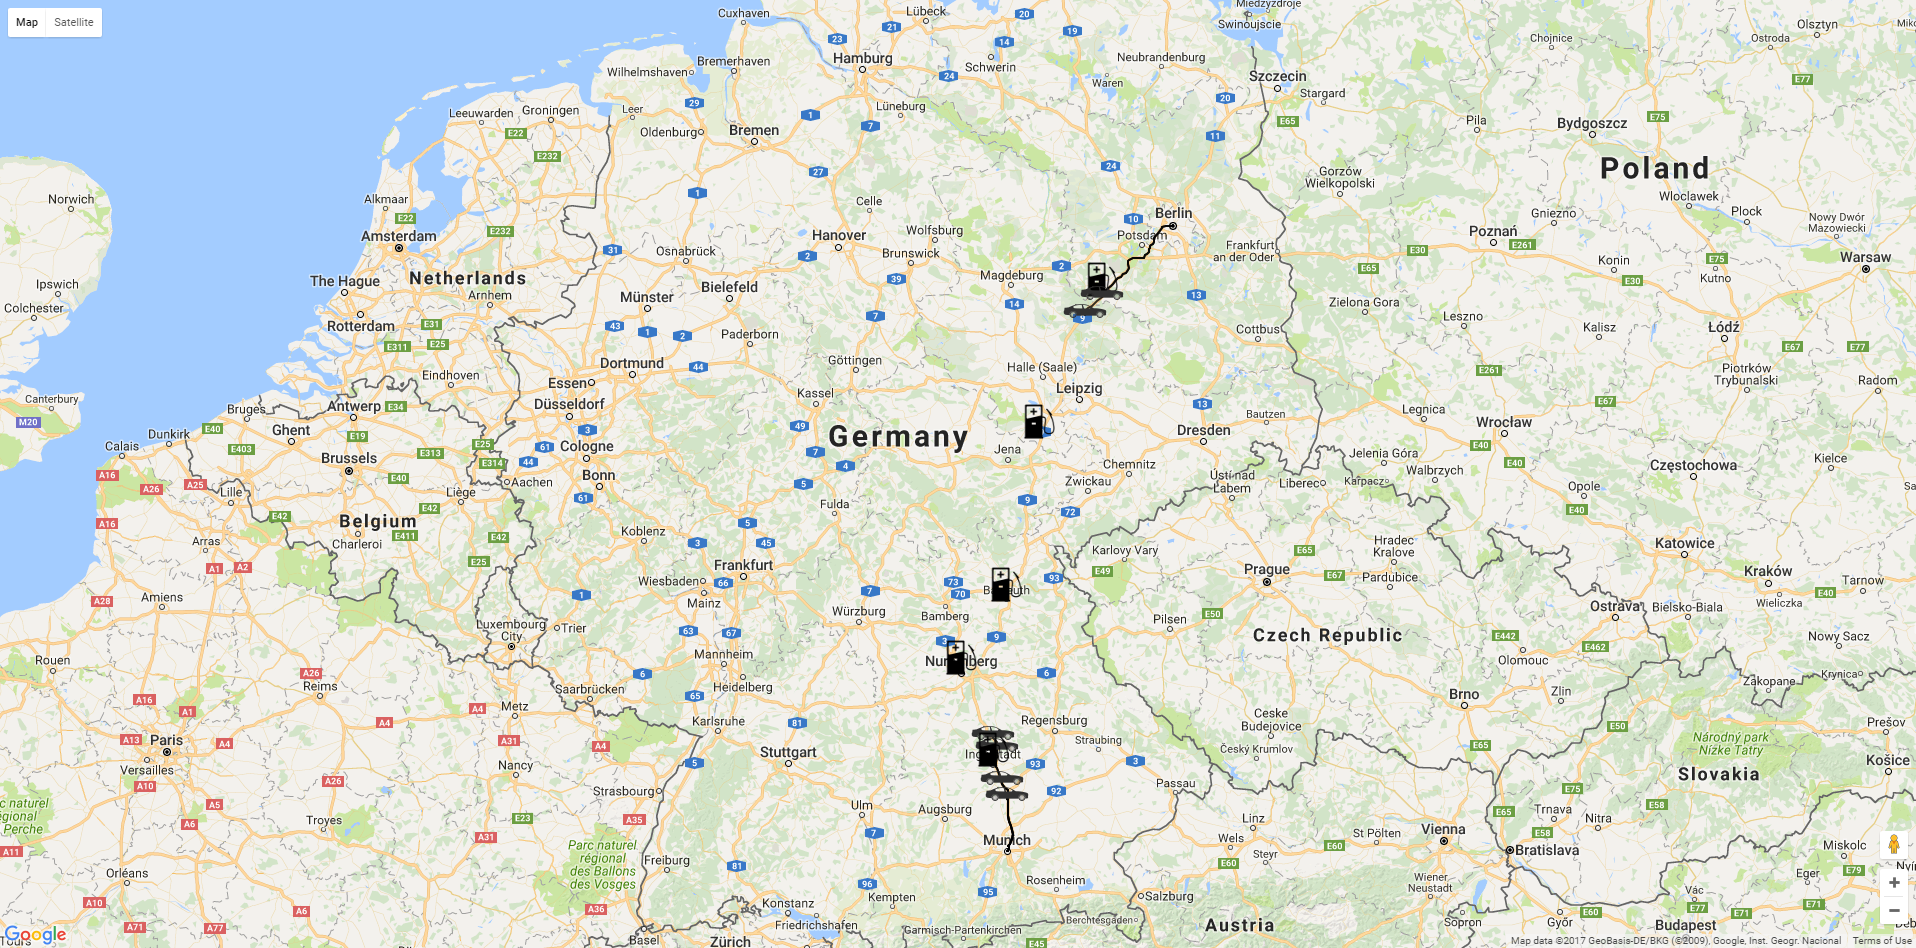
\includegraphics[width=\paperwidth]{images/simulation_manager.png}
\end{minipage}

\end{frame}
\clearpage



\begin{frame}[fragile]
\frametitle{config.js}

\begin{minted}{javascript}
var config = {
    mapID: "map",
    mapCenter: "Germany",
    mapZoom: 7,
    markers: {
        car: {
            url: "img/markers/car.png",
            anchor: new google.maps.Point(24, 18)
        },
        battery: {
            url: "img/markers/battery.png",
            anchor: new google.maps.Point(20, 36)
        }
    }
};
\end{minted}

\end{frame}
\clearpage



\begin{frame}[fragile]
\frametitle{main.js}

\begin{minted}{javascript}
$(document).ready(function () {

    // Init map
    var map = new Map();

    // Electric vehicles traveling from A to B
    var ev = [];

    ev.push(new EV(map.map, 1, 0, "Munich", "Berlin"));
    ev.push(new EV(map.map, 2, 10, "Munich", "Berlin"));
    ev.push(new EV(map.map, 3, 25, "Berlin", "Munich"));

    // Charging stations at location C
    var cs = [];

    cs.push(new CS(map.map, 1, "Ingolstadt"));
    cs.push(new CS(map.map, 2, "Nuremberg"));
    cs.push(new CS(map.map, 3, "Bayreuth"));
    cs.push(new CS(map.map, 4, "Osterfeld"));
    cs.push(new CS(map.map, 5, "Rabenstein"));
});
\end{minted}

\end{frame}
\clearpage